\section{ขั้นตอนวิธีเชิงตัวเลขพื้นฐาน}
\subsection{การดิสครีไทซ์เซชันแบบไฟไนต์ดิฟเฟอเรนจ์}

\hspace{1cm}ไฟไนต์ดิฟเฟอร์เรนจ์ (Finite Difference) คือวิธีการสำหรับการประมาณค่าอนุพันธ์เมื่อใช้วิธีเชิงตัวเลข ซึ่งในโครงงานวิจัยชิ้นนี้จะมีตัวดำเนินการที่เกี่ยวข้องกับอนุพันธ์ด้วยกัน 3 ตัวได้แก่ แกรเดียน ไดเวอร์เจน และ ลาปาเซียนซึ่งสามารถทำการหาได้ดังนี้

\subsubsection{การหาอนุพันธ์}

\hspace{1cm}ทั้ง แกรเดียน ไดเวอร์เจน และ ลาปาเซียน ล้วนมีพื้นฐานมาจากการหาค่าอนุพันธ์ในโครงงานวิจัยนี้จะใช้วิธีการฟอร์เวิร์ดดิฟเฟอร์เรนจ์ (Forward Difference) และใช้เงื่อนไขค่าขอบแบบนิวแมน (neumann boundary condition)

\noindent\hspace{1cm}นั่นคือการหาอนุพันน์ของค่าความเข้มที่พิกัดทางกายภาพเป็น $(i,j)$
\begin{align*}
	\frac{d}{dx} u_{i,j} = \frac{u_{i,j+1} - u_{i,j}}{h}
\end{align*}

เมื่อระบบกริดที่ใช้มีความห่างเพียงหนึ่งหน่วย จึงได้ว่า $h=1$ ทั้งนี้ระยะห่าง $h$ อาจเปลี่ยนไปตามชั้นของพีระมิดรูปภาพ

\begin{figure}[H]
    \centering
    \begin{subfigure}{0.95\linewidth}
        \centering
        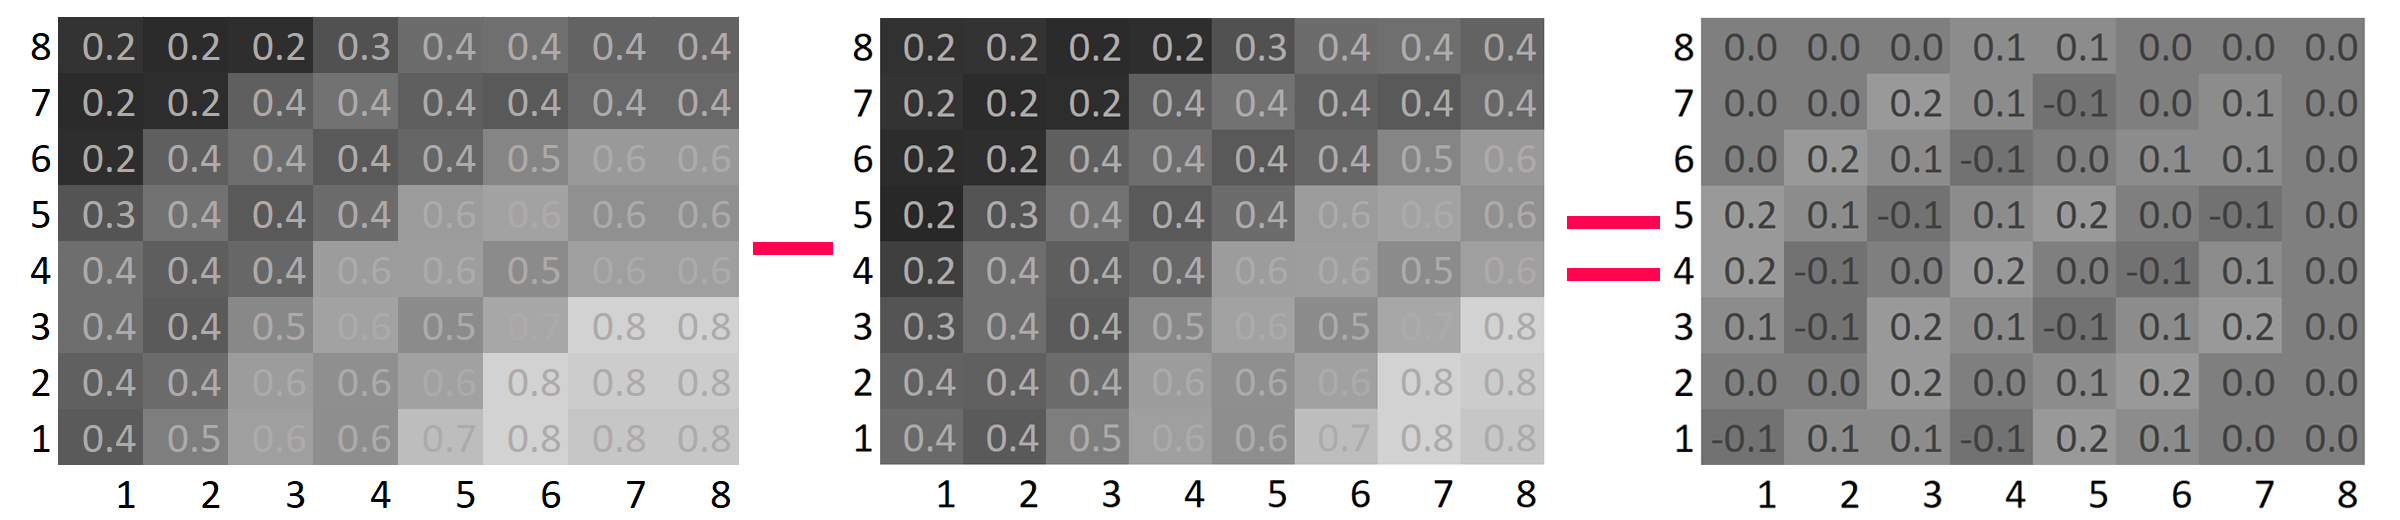
\includegraphics[width=0.9\linewidth]{image/finite_difference/x_derivertive.png}
    \end{subfigure}
    \caption{ตัวอย่างการหาอนุพันธ์บนภาพเฉดเทา}
    \label{figure:x-derivertive}
\end{figure}

\hspace{1cm} จากภาพ \ref{figure:grayscale-explain} เมื่อต้องการหาอนุพันธ์เทียบแกน x จะทำตามภาพที่ \ref{figure:x-derivertive}โดยทำการสร้างภาพซึ่งทำการตัดขอบทางซ้ายออกหนึ่งคอลัมม์และเพิ่มขอบทางขวาหนึ่งคอลัมม์โดยใช้เงื่อนไขค่าขอบแบบนิวแมน จากนั้นภาพที่สร้างขึ้นไปลบกับภาพเดิมจะได้อนุพันธ์ของภาพนั้นดังที่ปรากฏทางขวา ทั้งนี้หาก $ h \neq 1 $ สามารถทำการหารภาพผลลัพธ์ด้วยค่า $h$ ได้เพื่อให้ได้ค่าที่ต้องการ

\subsubsection{การหาแกรเดียน}
\noindent\hspace{1cm}สำหรับการหาแกรเดียน (Gradient) จะใช้การหาอนุพันธ์โดยวิธีฟอร์เวิร์ดดิฟเฟอร์เรนจ์ดังที่กล่าวไปในหัวข้อก่อนหน้า ั้งในแนวแกน x และแนวแกน y คำตอบที่ได้จะเป็นเวคเตอร์ของอนุพันธ์แนวแกน x และอนุพันธ์แนวแกน y  ได้เวคเตอร์ดังนี้ 

\begin{align*}
	\nabla \vec{v_{u_i}} = (\frac{d}{dx} u_{i,j},\frac{d}{dy} u_{i,j})^{\top}	
\end{align*}

\subsubsection{การหาไดเวอร์เจน}
\noindent\hspace{1cm}สำหรับไดเวอร์เจน (Divergence) จะเป็นการหาผลรวมของอนุพันธ์ในแต่ละแกนของเวคเตอร์ด้วยวิธีฟอร์เวิร์ดดิฟเฟอร์เรนจ์ นั่นคือ 

\begin{align*} 
	\nabla \cdot (\vec{v_{i,j}}) = \frac{\partial d}{\partial x}\vec{v_{i,j}}_x + \frac{\partial d}{\partial y}\vec{v_{i,j}}_y
\end{align*}

\subsubsection{การหาลาปาเชียน}
\noindent\hspace{1cm}สำหรับลาปาเซียน (Lapacian) นั่นคือการทำหาไดเวอร์เจรบนเวคเตอร์ที่หาแกรเดียนแล้ว แต่ทั้งนี้สามารถหาลาปาเชียนได้จาก

\begin{align*}
	\triangle u_{i,j} = u_{i-1,j} + u_{i+1,j} + u_{i,j-1} + u_{i,j+1} - 4 u_{i,j} 
\end{align*}

\subsection{ขั้นตอนวิธีเดินเวลา (explicit time marching method)}

\hspace{1cm} คณะวิจัย \cite{ref:ROF-template} ได้แนะนำวิธีการเชิงตัวเลขสำหรับการกำจัดสัญญาณรบกวนโดยใช้วิธีการเดินเวลาแบบชัดแจ้ง ซึ่งสามารถประยุกต์เป็นวิธีเชิงตัวเลขสำหรับการต่อเติมภาพได้ดังนี้
	
\hspace{1cm} เริ่มจากการแนะนําตัวแปรเวลาสังเคราะห์ (time artificial variable) จากนั้นหาคําตอบแบบสภาวะคงตัว (steady-state solution) ในขณะที่ $t\rightarrow \infty$ ของสมการเชิงอนุพันธ์ย่อยไม่เป็นเชิงเส้นที่ขึ้นอยู่กับเวลา 
\begin{align}
	u(\mathbf{x},t_{k+1})=u(\mathbf{x},t_{k})+\tau\left(\nabla \cdot\left(\dfrac{\nabla u (\mathbf{x},t_k)}{| \nabla u (\mathbf{x},t_k) | }\right) + \lambda(\mathbf{x})(u (\mathbf{x},t_k)-z(\mathbf{x})) \right),\ u(\mathbf{x},t_0)=z
	\label{e4}
\end{align}
เมื่อ $t_k=t_0+k\tau\ (\tau>0)$  แทนขั้นเวลาที่ $k$ และ $t_0=0$ แทนขั้นเวลาเริ่มต้น
	
 \vspace{0.5cm} \hspace{0.5cm}วิธีเดินเวลาแบบชัดแจ้งสำหรับภาพเฉดเทามีขั้นตอนวิธีดังนี้  \\
 
 % \vspace{0.5cm} 

\begin{algorithm}[H]
    \label{algorithm:explicit_timemarch}
    \caption{วิธีการเดินเวลาแบบชัดแจ้งสำหรับการต่อเติมภาพเฉดเทาที่ใช้การแปรผันรวม}
    \KwIn{
		\\
		\hspace{1cm} $u$ คือรูปภาพที่ต้องการต่อเติม \\
		\hspace{1cm} $\lambda$ คือพารามิเตอร์เร็กกิวลาร์ไรเซชัน ที่ได้กล่างถึงในสมการ (\ref{e2}) \\
		\hspace{1cm} $\beta$ เป็นจำนวนจริงบวกที่ใช้เพื่อหลีกเลี่ยงการหารด้วยศูนย์\\
		\hspace{1cm} $\tau$ เป็นจำนวนจริงบวกที่เป็นตัวแปรเดินเวลา \\
		\hspace{1cm} $N$ เป็นจำนวนเต็มบวกสำหรับกำหนดจำนวนรอบที่ทำงาน \\
		\hspace{1cm} $\varepsilon$ เป็นจำนวนจริงบวกของค่าความคลาดเคลื่อนสัมพัทธ์ \\
	}
	\KwOut{รูปภาพที่ผ่านการต่อเติมแล้ว}
    \SetKwFunction{FMain}{$u \longleftarrow ExplicitTimeMarching$}
    \SetAlgoNoLine 
    \SetKwProg{Fn}{}{}{}
    \Fn{\FMain{$u,\lambda,\beta,\tau,N,\varepsilon$}}{
        \textbf{initialize}
        $i = 0$; $z = u$; $err = 1$\\
        \While{$ i < N $ \textbf{and} $err > \varepsilon$}{
            $u^{old} = u$\\
            $u = u + \tau\left(\nabla \cdot\left(\dfrac{\nabla u}{\sqrt{u_x^2 + u_y^2+ \beta}}\right) + \lambda(u-z) \right)$ \\ 		
            $err = \frac{||u-u^{old}||}{||u||}$ \\
            $ i = i + 1 $
        }
    }
\end{algorithm}

\subsection{วิธีการทำซ้ำแบบจุดตรึง (fixed-point iteration method) }

\hspace{1cm} คณะวิจัย \cite{ref:FixpointSolver} ได้แนะนำวิธีการเชิงตัวเลขสำหรับการกำจัดสัญญาณรบกวนโดยใช้วิธีการทำซ้ำแบบจุดตรึง ซึ่งสามารถประยุกต์เป็นวิธีเชิงตัวเลขสำหรับการต่อเติมภาพได้ดังนี้
	
\hspace{1cm} เริ่มจากแนะนำดัชนีการทำซ้ำแบบจุดตรึง $\nu=0,1,2,\cdots$ และนิยามรูปแบบการทำซ้ำโดย
\begin{align}
	- \nabla\cdot\left(\dfrac{\nabla u^{[\nu+1]}}{{| \nabla u |}^{[v]} }\right) + \lambda(u^{[\nu+1]}-z)  = 0,\ u^{[0]}=z
	\label{e5}
\end{align}

\hspace{1cm} เนื่องจาก $\tfrac{1}{| \nabla u |}=\tfrac{1}{\sqrt{u_x^2+u_y^2}} \rightarrow \infty$ ในบริเวณที่ $u$ มีความเข้มสีเป็นเอกพันธ์ุ ($u(\mathbf{x})=$ ค่าคงตัว) เพื่อหลีกเลี่ยงปัญหาเชิงตัวเลขจะเกิดขึ้นใน (\ref{e4}) และ (\ref{e5}) เราจะใช้ 
\begin{align*}
|\nabla u| \approx| \nabla u |_\beta=\sqrt{u_x^2+u_y^2+\beta},\ 0< \beta \ll 1
 \end{align*}

\hspace{1cm}วิธีการทำซ้ำแบบจุดตรึงมีขั้นตอนดังนี้ \\
\vspace{0.5cm} 
\begin{algorithm}[H]
	\label{algorithm:fixedpoint}
	\SetAlgoNoLine
	\caption{วิธีการทำซ้ำจุดตรึงสำหรับการต่อเติมภาพเฉดเทาที่ใช้การแปรผันรวม}
	\KwIn{
		\\
		\hspace{1cm} $u$ คือภาพที่ได้รับการต่อเติม \\
		\hspace{1cm} $z$ คือภาพที่ต้องการต่อเติม \\
		\hspace{1cm} $\lambda$ คือพารามิเตอร์เร็กกิวลาร์ไรซ์เซชันในสมการ (\ref{e2}) \\
		\hspace{1cm} $\beta$ เป็นจำนวนจริงบวก\\
		\hspace{1cm} $N_{FP}$ เป็นจำนวนเต็มบวกสำหรับกำหนดจำนวนรอบการทำซ้ำจุดตรึง \\
		\hspace{1cm} $N_{GS}$ เป็นจำนวนเต็มบวกสำหรับกำหนดจำนวนรอบการทำซ้ำเกาส์-ไซเดล \\
		\hspace{1cm} $\varepsilon$ เป็นจำนวนจริงบวก\\
	}
	\KwOut{ภาพที่ผ่านการต่อเติมแล้ว}	
	\SetKwFunction{FMain}{$u \longleftarrow FixedPoint$}
	\SetKwProg{Fn}{}{}{}
	\Fn{\FMain{$u, z,\lambda, \beta, N_{FP}, N_{GS}, \varepsilon$}}{		
		\textbf{initialize} $i=0$;$u = z$;$err = 1 $\\
		\While{$ i < N_{FP} $ \textbf{and} $err > \varepsilon$}{
			$ u^{old} = u$ \\
			$D = \big[ D(u)_{i,j} \big] = \frac{1}{\sqrt{(u_x^2)_{i,j}+(u_y^2)_{i,j}+\beta}}, 1 \leq i \leq n_x, 1 \leq j \leq n_y$\\
			$u = GaussSeidel(u, z, D, \lambda, \beta, N_{GS})$\\
			$err = \frac{||u-u^{old}||}{||u||}$ \\
			$ i = i + 1 $
		}
	}
\end{algorithm}

\begin{algorithm}[H]
	\SetAlgoNoLine
	\caption{การทำซ้ำเกาส์-ไซเดล ภายในสำหรับวิธีการทำซ้ำจุดตรึง}
	\KwIn{
		\\
		\hspace{1cm} $u$ คือภาพที่ได้รับการต่อเติม\\
		\hspace{1cm} $z$ คือภาพที่ต้องการต่อเติม\\
		\hspace{1cm} $D$ คือสัมประสิทธิ์การแพร่กระจายไม่เป็นเชิงเส้น  \\
		\hspace{1cm} $\lambda$ คือพารามิเตอร์เร็กกิวลาร์ไรซ์เซชันในสมการ (\ref{e2}) \\
		\hspace{1cm} $\beta$ เป็นจำนวนจริงบวก\\
		\hspace{1cm} $N_{GS}$ เป็นจำนวนเต็มบวก \\
	}
	\KwOut{รูปภาพที่ผ่านการทำเกาส์-ไซเดลแล้ว}	
	\SetKwProg{Fn}{}{}{}
	\SetKwFunction{FMain}{$u \longleftarrow GaussSeidel$}
	\Fn{\FMain{$u, z, D, \lambda, \beta, N_{GS}$}}{
		\textbf{initialize} $k = 0$\\
		\While{$k < N_{GS}$}{
				$u_{i,j}^{k+1} = \frac{\lambda_{i,j}z_{i,j}+                (D_{i,j}(u_{i+1,j}^k+u_{i,j+1}^k)+D_{i-1,j}u_{i-1,j}^{k+1}+D_{i,j-1}u_{i,j-1}^{k+1})}{
				\lambda_{i,j}+(2D_{i,j}+D_{i-1,j}+D_{i,j-1})}$\\
				$k = k+1$
		}
	}
\end{algorithm}
\vspace{0.5cm}
\hspace{1cm} จาก (\ref{e4}) และ (\ref{e5}) เราพบว่ายิ่ง $\beta$ มีค่าน้อยลงมากขึ้นเท่าไหร่ ความแม่นยำของตัวแบบ (\ref{e1}) ยิ่งมีมากขึ้นเท่านั้น นอกจากนี้ เรายังพบอีกว่า การแก้สมการ (\ref{e4}) และ (\ref{e5}) ยิ่งมีความยุ่งยากมากขึ้นสำหรับ $\beta$ ที่มีค่าน้อยๆ 

\hspace{1cm} เพื่อเอาชนะความยากเชิงตัวเลขนี้ คณะวิจัยโดย \cite{ref:splitbergman-inpaint} ได้แนะนำวิธีการสปริทเบรกแมนซึ่งสามารถกล่าวถึงพอสังเขป ดังนี้

\subsection{วิธีการสปริทเบรกแมน (Split Bregman method)}

\hspace{1cm} เริ่มจากการแนะนำเวกเตอร์เสริม $\boldsymbol{w}$ พารามิเตอร์เบรกแมน (Bregman parameter) $\boldsymbol{b}$ และพารามิเตอร์เพนัลที (panalty parameter) $\theta>0$ และเขียน (\ref{e1}) ใหม่ ดังนี้
\begin{align}
	\min_{u,\boldsymbol{w}} \{ \mathcal{J}(u,\boldsymbol{w}) = \dfrac{1}{2} \int_{\Omega} \lambda(u-z)^2 d\Omega +  \int_{\Omega}  | \boldsymbol{w}|  d\Omega + \frac{\theta}{2} \int_{\Omega} (\boldsymbol{w} - \nabla u + \boldsymbol{b}) d\Omega \}
	\label{e6}
\end{align}
\hspace{1cm}สำหรับการหาคำตอบของ (\ref{e6}) เราจะใช้วิธีการหาค่าต่ำที่สุดแบบสลับ (alternating minimization method) โดยเริ่มจากการตรึง $\boldsymbol{w}^{\text{old}}$ และ $\boldsymbol{b}^{\text{old}}$ จากนั้นแก้ปัญหาย่อยสำหรับ $u$
\begin{align}
	u^{\text{New}}=\underset{u}{\arg\min} \{ \mathcal{J}_1(u) = \dfrac{1}{2} \int_{\Omega} \lambda(u-z)^2 d\Omega + \frac{\theta}{2} \int_{\Omega} (\boldsymbol{w}^{\text{old}} - \nabla u + \boldsymbol{b}^{\text{old}}) d\Omega \}
	\label{e7}
\end{align}
ต่อไปใช้ $u^{\text{New}}$ ที่ได้จากการแก้ปัญหาย่อย (\ref{e7}) เพื่อแก้ปัญหาย่อยสำหรับ $\boldsymbol{w}$
\begin{align}
	\boldsymbol{w}^{\text{New}}=\underset{\boldsymbol{w}}{\arg\min} \{ \mathcal{J}_2(\boldsymbol{w}) = \int_{\Omega}  |\boldsymbol{w}|  d\Omega  + \frac{\theta}{2} \int_{\Omega} (\boldsymbol{w} - \nabla u^{\text{New}} + \boldsymbol{b}^{\text{old}}) d\Omega \}
	\label{e8}
\end{align}
	สุดท้ายจึงปรับปรุงพารามิเตอร์เบรกแมนโดย 
\begin{align}
	\boldsymbol{b}^{\text{New}}=\boldsymbol{b}^{\text{old}}+\nabla u^{\text{New}}-\boldsymbol{w}^{\text{New}}
	\label{e9}
\end{align}
ดำเนินการเช่นนี้จนกระทั่ง $||u^{\text{new}}-u^{\text{old}}||< \epsilon_1$ หรือ $\text{New}>\epsilon_2$ เมื่อ $\epsilon_1,\epsilon_2>0$ \\ 
\vspace{0.5cm}
\hspace{1cm}วิธีการสปริทเบรกแมนมีขั้นตอนวิธีดังนี้ \\
\vspace{0.5cm}
\begin{algorithm}[H]
    \SetAlgoNoLine
    \caption{วิธีสปริทเบรกแมนสำหรับการต่อเติมภาพที่ใช้การแปรผันรวม}
    \SetKwFunction{FMain}{$u \longleftarrow SplitBregman$}
    \SetKwProg{Fn}{}{}{}
    \KwIn{
		\\
		\hspace{1cm} $u$ คือรูปภาพที่ต้องการต่อเติม \\
		\hspace{1cm} $\lambda$ คือพารามิเตอร์เร็กกิวลาร์ไรเซชัน ที่ได้กล่างถึงในสมการ (\ref{e2}) \\
        \hspace{1cm} $\theta$ คือพารามิเตอร์เพนัลที ซึ่งเป็นจำนวนจริงบวก\\
        \hspace{1cm} $N_{gs}$ เป็นจำนวนเต็มบวกสำหรับกำหนดจำนวนรอบที่ทำงานของการทำเกาส์-ไซเดล \\
		\hspace{1cm} $N$ เป็นจำนวนเต็มบวกสำหรับกำหนดจำนวนรอบที่ทำงานของสปริทเบรกแมน \\
		\hspace{1cm} $\varepsilon$ เป็นจำนวนจริงบวกของค่าความคลาดเคลื่อนสัมพัทธ์ \\
	}
	\KwOut{รูปภาพที่ผ่านการต่อเติมแล้ว}	
    \Fn{\FMain{$u,\lambda, \theta, N_{gs}, N, \varepsilon$}}{
        \textbf{initialize}
        $i = 0$,
        $\boldsymbol{b} = \vec{0}$,
        $\boldsymbol{w} = \vec{0}$,
        $z = u$ \\
        \While{$ i < N $ \textbf{and} $err > \varepsilon$}{
            $u^{old} = u$; 
            $w^{old} = w$;
            $b^{old} = b$;
             \\
            $u^{new}=\underset{u}{\arg\min} \{ \mathcal{J}_1(u) = \dfrac{1}{2} \int_{\Omega} \lambda(u-z)^2 d\Omega + \frac{\theta}{2} \int_{\Omega} (\boldsymbol{w}^{\text{old}} - \nabla u + \boldsymbol{b}^{\text{old}}) d\Omega \}$ \\
            $w^{new} =\underset{\boldsymbol{w}}{\arg\min} \{ \mathcal{J}_2(\boldsymbol{w}) = \int_{\Omega}  | \boldsymbol{w}|  d\Omega  + \frac{\theta}{2} \int_{\Omega} (\boldsymbol{w} - \nabla u^{\text{New}} + \boldsymbol{b}^{\text{old}}) d\Omega \}$\\
            $ b^{new} = b^{old} + \nabla u^{new} - \boldsymbol{w}^{new} $ \\
            $err = \frac{||u^{new}-u^{old}||}{||u^{new}||}$ \\
            $ i = i + 1 $ \\
        }
    }
\end{algorithm}
\vspace{0.5cm}
\textbf{หมายเหตุ:}
\begin{itemize}
	\item [(1)] ผลเฉลยของ $ u = \underset{u}{\arg\min} \mathcal{J}_1(u) $ กำหนดโดยการแก้ปัญหาผลเฉลยของ
	 $$ - \theta \triangle u + \lambda u = \lambda z - \theta \nabla \cdot (\boldsymbol{w}-\boldsymbol{b})$$ 
	 โดยใช้วิธีการไฟไนต์ดิฟเฟอเรนจ์และวิธีการเกาส์-ไซเดลจำนวน $N_{gs}$ รอบ
	\item [(2)] ผลเฉลยของ $ \boldsymbol{w} = \underset{\boldsymbol{w}}{\arg\min} \mathcal{J}_2(\boldsymbol{w}) $ กำหนดโดย $$\boldsymbol{w} = max\bigg\{(\nabla u + \boldsymbol{b}) - \frac{1}{\theta},0\bigg\}$$
\end{itemize}